\section{Parallel versions}

\subsection{Native threads}
The goal of the parallel version is to sort the global array, by splitting the array in chunks to give to each thread. Every thread needs to run the odd and the even phase on its partition, and it also needs to consider its neighbors (otherwise it would perform a local sorting, not a global one). The ``odd-even'' function is the one to be mapped, and its parameters are the bounds (fixed for each thread) and the phase (odd or even).

\paragraph{Data partitioning}
The simplest division of the work is the static block distribution. Each thread (except for the last one) shares its last element with another thread. If the array has $n$ elements and there are $nw$ workers, I have $nw - 1$ overlapping points. It's like I have to split $n + nw - 1$ elements among $nw$ workers. Simplifying, the average chunk length is $\frac{n - 1}{nw} + 1$ (if $n - 1$ is not divisible by $nw$, the remaining elements will be distributed uniformly). Here is an example with $n = 10$ and $nw = 4$.

\begin{center}
	\begin{figure}[ht!]
		\makebox[\textwidth]{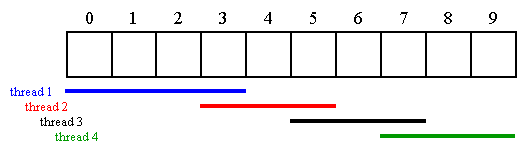
\includegraphics[width=0.55\paperwidth]{img/array.pdf}}
		\caption{Work division.} \label{array}
	\end{figure}
\end{center}
Some testing has proven the work to be well-balanced in this way, with an average difference of workload of 4.31\% among threads; hence I didn't consider any form of dynamic load balancing, such as job stealing.

Since the threads work on contiguous partitions of the same global array, there might be \textit{false sharing} problems, that will be discussed later on.

Each phase is trivial to parallelize, but the switch from one phase to the next one requires a synchronization between the threads. If the two phases are synchronized, it is not possible that two threads work on the same element at the same time. This can be noticed for example by simulating an odd phase and an even phase in figure \ref{array}.

\paragraph{Barriers}
To synchronize the threads, a solution is to use barriers. The best solution in term of performances has proven to be to use as many barriers as many iterations the algorithm would do (an upper bound is given by the size of the array, since the odd-even sort is a parallel version of the bubble sort). A slightly slower solution is the one with only a single reusable barrier, that involves two atomic variables (one for the current thread count, and one for the count of the ``generations''). The slowest solution is the one with mutexes and condition variables, because of the overhead of descheduling.

\paragraph{Developing the parallel version}
The first parallel version was based on a pool of workers, each one with its pointer to the global array, moved by an offset. Every thread executes the odd and even phase, separated by a barrier, then adds its total number of swaps to the global atomic variable: that variable quickly becomes the bottleneck, since every operation takes a lock on the memory bus, increasing the serial fraction of the program. The threads exit from the loop when there are no swaps in the global variable (if there is any swap in the local phase, there's no need for that thread to read the global variable). Every iteration goes on following this schema:
\begin{verbatim}
    execute odd phase
    barrier
    execute even phase
    update global swaps
    barrier
    check exit condition
    barrier
    reset global swaps
\end{verbatim}

In the second version I avoided the bottleneck of the global atomic variable by using a shared vector in which every thread writes its number of swaps; the vector was padded to the cache line to avoid false sharing. The switch from the first to the second phase is synchronized among the workers. Then I added a ``controller'' thread, to speed up the switch to the next iteration (from the end of the second phase to the first again): the controller reads in a tight loop the swaps array, and if there is at least a swap, it immediately decreases the value of another barrier, shared among the workers and the controller. In this way, in most cases (non-exit situations), the workers have only to wait the last worker to restart another iteration, without any overhead to sum or check the global number of swaps. This had a good impact on the performance, and also reduced the number of barriers from 3 to 2, since there's no need to wait that all threads have modified the global variable. To avoid false sharing, the array is padded to the cache line size (if not given as an argument, it's assumed to be 64 bytes).

\paragraph{Possible false sharing}
Another try was to avoid the possible false sharing on the global array between adjacent threads, so I made the threads to work on a local copy of their portion of the array, synchronizing themselves with the rightmost element (the one shared with the next worker). This solution had slightly worse performances, probably because the false sharing was not a problem at all: in fact, the threads run at almost the same speed (as said in the load balancing considerations) from left to right, hence when a thread arrives to its rightmost part, the neighbor is no more working on that side of the array. I'm assuming that the portions are big enough to not fit in a L1 cache line (with cache lines of 64 bytes and elements of 4 bytes, at least 16 elements). The time spent for the copy of the array was negligible.

\paragraph{Final version}
This version uses only one barrier, needed to synchronize the threads on the exit condition, or to continue another odd-even phase. I was able to remove the barrier between the odd and the even phase because there's no really need that all the threads wait the end of the first phase: it's sufficient that every thread waits the end of its neighbors. When a thread finishes the odd phase, it enters in a ``ready state'' by increasing a counter in the phases array, and when its neighbors are also in that state, it can safely start the even phase. This asynchronous transition from the odd to the even phase allowed the program to run faster. Also this array is padded to the cache line to avoid false sharing.

To avoid the optimizer to optimize (badly) the active waiting loop, I have used the assembly \texttt{nop} instruction instead of a semicolon, otherwise the value of the neighbor would never be updated after the first iteration, blocking the program in an infinite loop. This can also be avoided by using an array of \texttt{volatile} variables.

Since the work is well-balanced among the workers, the bottleneck was the atomic variable for the barrier, and not the waiting for slower threads.

\paragraph{Thread pinning}
Since the Xeon for the tests has no MCDRAM installed, and therefore its mesh is configured with the ``all-to-all" clustering mode, for the thread pinning I chose a linear mapping, putting one thread per core, from 1 to 64. With my data partitioning threads with adjacent thread IDs have adjacent array partitions, and since the L2 cache is shared between two cores (0-1, 2-3, \dots), this linear mapping maximizes the sharing of the cache.

\paragraph{Performances}
Here are the results of speedup and efficiency, tested on array from 100K to 600K elements. Smaller arrays are not considered because of the relatively small execution time also with the sequential version (e.g. sorting sequentially 50K elements takes less than one second). With the basic 128 bit vectorization, I was able to reach higher speedups on few elements (17x on 100K elements). Why? Because the total execution time was 4 times higher than the 512 bit vectorized version, hence the fixed overheads were more hidden. Probably, a 4 times bigger L1 cache would help to achieve higher speedups, by keeping keep the same ``vectorization vs. L1 cache size'' ratio and reducing the overhead of prefetching, but some overheads are fixed and cannot be reduced in this way, like the atomic barrier.

We can notice a superlinear behavior when the partitions have comparable size with the L1 cache (32KB per core, 8K C++ 32-bit integers), but also the global problem size is important, because the odd-even sort is a quadratic algorithm, not a linear one (if I double the problem size, I have more than the double of the work to hide overheads with).
\bigbreak

\begin{figure}[ht!]
    \centering
    \begin{tikzpicture}
        \pgfplotstableread{data/speedup_native.dat}{\file}
        \begin{axis}[style,
            ymax = 64,
            ytick distance=5,
            xlabel={Number of workers},
            ylabel={Speedup},
            legend pos=outer north east
            ]
            \addplot [black, thick] table [x={x}, y={ideal}] {\file}; \addlegendentry{Ideal};
            \addplot table [x={x}, y={100}] {\file}; \addlegendentry{100K};
            \addplot table [x={x}, y={200}] {\file}; \addlegendentry{200K};
            \addplot table [x={x}, y={300}] {\file}; \addlegendentry{300K};
            \addplot table [x={x}, y={400}] {\file}; \addlegendentry{400K};
            \addplot table [x={x}, y={500}] {\file}; \addlegendentry{500K};
            \addplot table [x={x}, y={600}] {\file}; \addlegendentry{600K};
        \end{axis}
    \end{tikzpicture}
    \caption{Speedup of the native threads version}
\end{figure}

\begin{figure}[ht!]
    \centering
    \begin{tikzpicture}
        \pgfplotstableread{data/efficiency_native.dat}{\file}
        \begin{axis}[style,
            ymax = 2,
            xlabel={Number of workers},
            ylabel={Efficiency},
            legend pos=outer north east,
            ]
            \addplot [black, thick] table [x={x}, y={ideal}] {\file}; \addlegendentry{Ideal};
            \addplot table [x={x}, y={100}] {\file}; \addlegendentry{100K};
            \addplot table [x={x}, y={200}] {\file}; \addlegendentry{200K};
            \addplot table [x={x}, y={300}] {\file}; \addlegendentry{300K};
            \addplot table [x={x}, y={400}] {\file}; \addlegendentry{400K};
            \addplot table [x={x}, y={500}] {\file}; \addlegendentry{500K};
            \addplot table [x={x}, y={600}] {\file}; \addlegendentry{600K};
        \end{axis}
    \end{tikzpicture}
    \caption{Efficiency of the native threads version}
\end{figure}


\clearpage


\subsection{FastFlow}
The parallel version developed with FastFlow is very simple: I used a farm with feedback loop and no collector, where each thread is statically assigned a portion of the array at the moment of its creation; the emitter sends a dummy task just to tell that they can run another phase of the sorting. Each worker performs one phase of the sorting and sends back to the emitter its number of swaps, and after two consecutive phases with no swaps from anyone, the emitter stops the workers. The main bottleneck is the message passing, because this solution is logically identical to the one with two barriers and one controller thread, but performs worse.

\paragraph{Alternative versions}
To mimick the asynchronous behavior of the native threads version, I modified the emitter to keep track of the current phase of the workers and the one that they are eventually ready for, unlocking as soon as possible all the workers that have finished and whose neighbors are in a ``ready state'', recursively, but unfortunately the extra centralized logic slowed down the entire computation: the workers are balanced and they end their computation more ore less simultaneously: a broadcast message is much faster.

\paragraph{Fine tuning}
To reduce the overheads, the workers don't send a dynamically allocated element to the emitter, but they send the pointer to their struct-local variable. This improved the performance by 10\%. I can do it safely because the variable goes only to the emitter, and the next svc call of that worker will happen only after that the emitter read the value.

The same does the emitter, by sending a dummy pointer that will never be read from the workers.

Finally, by moving the variables of the emitter from the struct to the \texttt{svc} method through the \texttt{static} qualifier, I obtained a 0.5\% of performance improvement.

I tried the queues in blocking mode and no default thread mapping, and as expected I obtained worse performances in both cases.
\bigbreak

Here are the speedup and efficiency plots of the FastFlow version. For a better comparison, I kept the same scale of the previous plots.

\begin{figure}[ht!]
    \centering
    \begin{tikzpicture}
        \pgfplotstableread{data/speedup_ff.dat}{\file}
        \begin{axis}[style,
            ymax = 64,
            ytick distance=5,
            xlabel={Number of workers},
            ylabel={Speedup},
            legend pos=outer north east
            ]
            \addplot [black, thick] table [x={x}, y={ideal}] {\file}; \addlegendentry{Ideal};
            \addplot table [x={x}, y={100}] {\file}; \addlegendentry{100K};
            \addplot table [x={x}, y={200}] {\file}; \addlegendentry{200K};
            \addplot table [x={x}, y={300}] {\file}; \addlegendentry{300K};
            \addplot table [x={x}, y={400}] {\file}; \addlegendentry{400K};
            \addplot table [x={x}, y={500}] {\file}; \addlegendentry{500K};
            \addplot table [x={x}, y={600}] {\file}; \addlegendentry{600K};
        \end{axis}
    \end{tikzpicture}
    \caption{Speedup of the FastFlow version}
\end{figure}

\begin{figure}[ht!]
    \centering
    \begin{tikzpicture}
        \pgfplotstableread{data/efficiency_ff.dat}{\file}
        \begin{axis}[style,
            ymax = 2,
            xlabel={Number of workers},
            ylabel={Efficiency},
            legend pos=outer north east,
            ]
            \addplot [black, thick] table [x={x}, y={ideal}] {\file}; \addlegendentry{Ideal};
            \addplot table [x={x}, y={100}] {\file}; \addlegendentry{100K};
            \addplot table [x={x}, y={200}] {\file}; \addlegendentry{200K};
            \addplot table [x={x}, y={300}] {\file}; \addlegendentry{300K};
            \addplot table [x={x}, y={400}] {\file}; \addlegendentry{400K};
            \addplot table [x={x}, y={500}] {\file}; \addlegendentry{500K};
            \addplot table [x={x}, y={600}] {\file}; \addlegendentry{600K};
        \end{axis}
    \end{tikzpicture}
    \caption{Efficiency of the FastFlow version}
\end{figure}
